
\setcounter{secnumdepth}{4}

\titleformat{\paragraph}
{\normalfont\normalsize\bfseries}{\theparagraph}{1em}{}
\titlespacing*{\paragraph}
{0pt}{3.25ex plus 1ex minus .2ex}{1.5ex plus .2ex}

\section{Analysis of Saving and Loan Accounts Data}
In this we will discuss about the work on a 1999 Czech Financial Data-set with real anonymized transactions \cite{19}. The aim was to learn the concept of ALM for banks and for that purpose we tried to simulate the ALM portfolio based on the given data set. As depicted in Figure 1.3 ALM Cycle of a Bank, the saving account deposits are the liability to the bank and the loans are assets for the bank. While neglecting all other parameters of the bank we are considering just deposits and loan to simulate the ALM concept.


\section{Dataset Description}
The dataset consists of 8 files in it, but we will be using only two namely transaction and loan. The description of both the files is as follows:

\begin{itemize}
\item \textbf{Relational Transaction: }This file consist of 1056320 rows, where each row is a transaction to an account. The attributes of the transaction file are :

\item[1.] Trans id: unique transaction number.
\item[2.] Account id: unique account number.
\item[3.] Date: date of the transaction.
\item[4.] Type: type of transaction: credit or debit.
\item[5.] Operation: mode of transaction: credit card withdrawal, credit in cash, collection from another bank, withdrawal in cash, remittance to another bank.
\item[6.] Amount: Transaction amount
\item[7.] Balance: remaining balance after transaction

\item \textbf{Relational Loan: }This file consist of 682 rows, where each row is a loan given per account. The attributes of the loan file are :

%\begin{enumerate}
\item[1.] Account id: unique account number.
\item[2.] Date: date of the transaction.
\item[3.] Amount :loan amount
\item[4.] Duration: Duration of loan 
\item[5.] Payment: amount to be paid monthly.
\item[6.] Status : Loan account status: cleared loan, client in debt, defaulter, paying loan
\end{itemize}
The overview of the transaction file is as follows:
				\begin{center}
				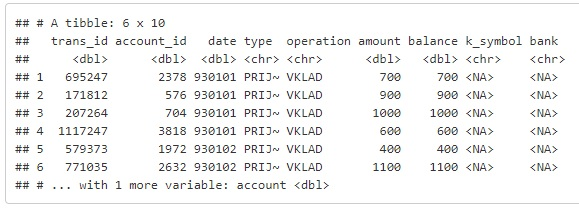
\includegraphics[width=\linewidth]{figures/description-transaction.jpg}	
				\captionof{figure}{Description of Transaction File}
				\label{fig: Description of Transaction File}
				\end{center}
The summary of the transaction file is as follows:
				\begin{center}
				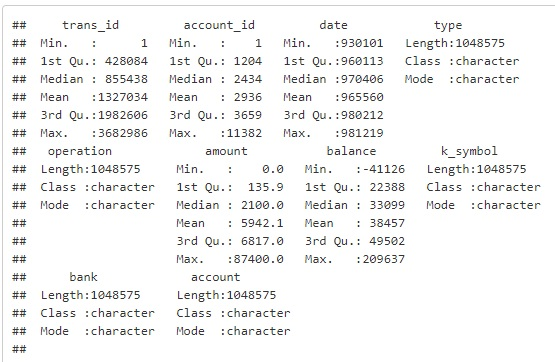
\includegraphics[width=\linewidth]{figures/summary-transaction.jpg}	
				\captionof{figure}{Description of Transaction File}
				\label{fig: Description of Transaction File}
				\end{center}

The overview of the loan file is as follows:
				\begin{center}
				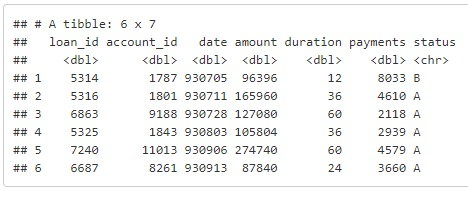
\includegraphics[width=\linewidth]{figures/description-loan.jpg}	
				\captionof{figure}{Description of Loan File}
				\label{fig: Description of Loan File}
				\end{center}
The summary of the loan file is as follows:
				\begin{center}
				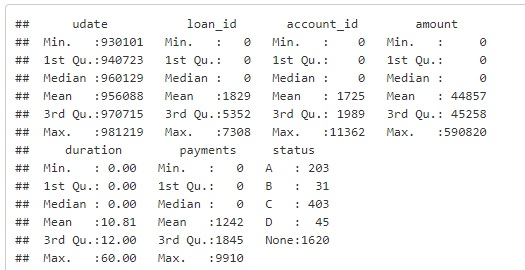
\includegraphics[width=\linewidth]{figures/summary-loan.jpg}	
				\captionof{figure}{Description of Loan File}
				\label{fig: Description of Loan File}
				\end{center}



\section{Simulation of the Experiment}

\begin{algorithm}[H]

\caption{Pseudo Code for Computation of Maturity Table for ALM}

\begin{algorithmic}[1] 
						
\STATE Initialization:\\
Start $\gets$ [The starting day of each time bucket] \\
End $\gets$ [The ending day of each time bucket] \\
i $\gets$ 0\\
max $\gets$ length(Start)\\

\STATE \emph{while(i < max)}:

\STATE \tab \begin{equation}
Liability = \Sigma_{j = Start[i]}^{End[i]} deposit\_amount[j]
\end{equation}

\STATE \tab \begin{equation}
Asset[i] = \Sigma_{j = Start[i]}^{End[i]} loan\_amount[j]
\end{equation}

\STATE \tab \begin{equation}
Withdrawal[i] = \Sigma_{j = Start[i]}^{End[i]} withdrawal\_amount[j]
\end{equation}

\STATE \tab \begin{equation}
Mismatch[i] = Asset[i] - Withdrawal[i] 
\end{equation}

\STATE \tab \begin{equation}
\%\_Mismatch[i] = \frac{Mismatch[i]}{Liability[i]}
\end{equation}

\STATE Cumulative \% Mismatch = Cumulative\_Sum(\%\_Mismatch)

\end{algorithmic}

\end{algorithm}

\section{Results of the Experiment}


\begin{table}[h!]
  \begin{center}
    \caption{Results of the ALM Simulation 1}
    \label{tab:Results of the ALM Simulation 1}
    \begin{tabular}{l|l|l|l|l} % <-- Alignments: 1st column left, 2nd middle and 3rd right, with vertical lines in between
      \hline
      \textbf{\#Start} & \textbf{\#End} & \textbf{Liability}& \textbf{Withdrawal}& \textbf{Assets} \\
	\hdashline
	\hdashline
      1 & 1 & 3200 & 0  & 0 \\
	\hline
      2 &  7 & 28964 & 0 & 0\\
	\hline
      8 & 14 & 268887 & 0 & 0 \\
	\hline
      15 & 28 & 296622 & 0 & 0 \\
	\hline
      29 & 90 & 5182037 & 1166308 & 0 \\
	\hline
      91 & 180 & 10425204 & 13085553 & 0 \\
	\hline
      181 & 365 & 24532470 & 64642130 & 2619276 \\
	\hline
      366 & 1095 & 91889223 & 577121716 & 26724276 \\
	\hline
      1096 & 1825 & 197436280 & 1261537518 & 48700920 \\
	\hline
      1826 & 2179 & 109423887 & 832618418 & 25217268  \\

	\hdashline
	\hdashline
	\multicolumn{5}{l}{\#Start: Starting day of time bucket} \\
	\multicolumn{5}{l}{\#End: Ending day of time bucket} \\
	\multicolumn{5}{l}{Liability: Total amount deposited in each time bucket} \\
	\multicolumn{5}{l}{Withdrawal: Total amount withdrawn from deposited amount in each time bucket} \\
	\multicolumn{5}{l}{Assets: Total loan amount granted in each time bucket} \\
	\hline
    \end{tabular}
  \end{center}
\end{table}


\begin{table}[h!]
  \begin{center}
    \caption{Results of the ALM Simulation 2}
    \label{tab:Results of the ALM Simulation 2}
    \begin{tabular}{l|l|l|l|l} % <-- Alignments: 1st column left, 2nd middle and 3rd right, with vertical lines in between
      \hline
      \textbf{\#Start} & \textbf{\#End} & \textbf{Mismatch}& \textbf{\% Mismatch}& \textbf{Cumulative \% Mismatch}\\
	\hdashline
	\hdashline
      1 & 1 &  -3200 & -100.00000 & -100.0000 \\
	\hline
      2 &  7 & -28964 & -100.00000 & -200.0000  \\
	\hline
      8 & 14 & -268887 & -100.00000 & -300.0000  \\
	\hline
      15 & 28 & -296622 & -100.00000 & -400.0000  \\
	\hline
      29 & 90 & -5181863 & -99.99665 & -499.9966  \\
	\hline
      91 & 180 & -10423808 & -99.98661 & -599.9833  \\
	\hline
      181 & 365 & -21012942 & -85.65359 & -685.6368    \\
	\hline
      366 & 1095 & -47153606 & -51.31571 & -736.9526    \\
	\hline
      1096 & 1825  -109674289 & -55.54921 & -792.5018   \\
	\hline
      1826 & 2179 & -55699964 & -50.90293 & -843.4047  \\

	\hdashline
	\hdashline
	\multicolumn{5}{l}{Mismatch: Difference in assets and liabilities} \\
	\multicolumn{5}{l}{\% Mismatch: Mismatch as \% to outflow i.e. liability} \\
	\multicolumn{5}{l}{Cumulative \% Mismatch: Cumulative sum of \% Mismatch} \\
	\hline
    \end{tabular}
  \end{center}
\end{table}

\section{Analysis of the Results}

As per the RBI guidelines the negative cumulative mismatch in the first four buckets should not exceed 5\%, 10\%, 15\% and 20\% of the cash outflow of the respective time bucket.
Here a lot of parameters are from the ALM sheet are missing that's why the cumulative mismatch is not matching.\\

Although the difference between the liability and the withdrawal column is significantly positive the customers are not withdrawing all the amount deposited in the account. This lead for us to investigate more on the data .

\subsection{Post Result Analysis of Data}

Here we have assumed the different window for the transaction amount and the frequency of the transactions in that amount window is as follows:

\begin{table}[h!]
  \begin{center}
    \caption{The amount window and frequency of transactions}
    \label{tab:The amount window and frequency of transactions}
    \begin{tabular}{l|l|l} % <-- Alignments: 1st column left, 2nd middle and 3rd right, with vertical lines in between
      \hline
      \textbf{Sr. No.} & \textbf{Window} & \textbf{Frequency}\\
	\hdashline
	\hdashline
      1  &     [0,100) & 218988\\
	\hline
	2  &   [100,500) & 160913\\
	\hline
	3  & [500,1e+03) & 48191\\
	\hline
	4  & [1e+03,1e+04) & 423892\\
	\hline
	5 &  [1e+04,2e+04) & 104482\\
	\hline
	6 &  [2e+04,5e+04) & 88270\\
	\hdashline
	\hline
    \end{tabular}
  \end{center}
\end{table}

The frequency density plot of the above table looks like this:
				\begin{center}
				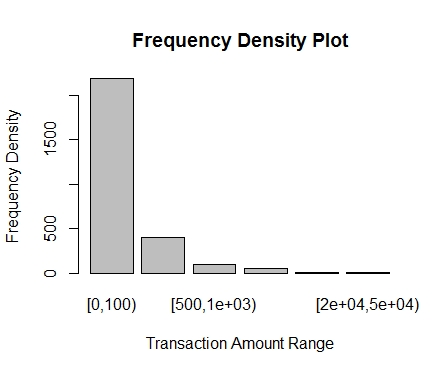
\includegraphics[width=\linewidth]{figures/freq-density-plot.jpeg}	
				\captionof{figure}{Frequency density plot of the Transaction Amount}
				\label{fig: Frequency density plot of the Transaction Amount}
				\end{center}

The plot seems to be following Pareto distribution, which means that 80\% of the transactions belong to the first window.  Lets again select the random account numbers and plot their deposits and withdrawal transactions. 
				\begin{center}
				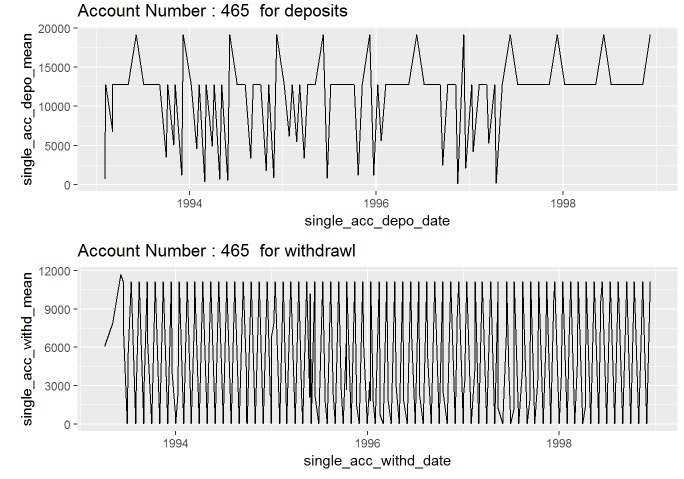
\includegraphics[width=\linewidth]{figures/deposit-withdrawal-plot.jpg}	
				\captionof{figure}{The deposit and withdrawal plot for randomly chosen account number}
				\label{fig: The deposit and withdrawal plot for randomly chosen account number}
				\end{center}
The plot shows that the mean amount deposited is maximum than mean amount withdrawal and the frequency of deposits is less than the frequency of withdrawal. But there were some cases where this condition failed. After analyzing such more plots we can say that there will always be some amount remaining in the account. The bank can focus on such customers and encourage them to invest in their various investment schemes, so that this money can be utilized as asset for some fixed duration of time.\\ 
The formula for finding the assets from each saving accounts can be given as:
\begin{equation}
Assets from Saving Account = \{Average Amount Deposited - Average Amount Withdrawal\}_{over given time bucket}
\end{equation}

\section{Conclusion}

In this chapter, we have simulated the concept of ALM for banks and analyzed the data for getting some meaningful insights. 


